			


%#############################################################################
%
%              						CHAPTER 
%
%#############################################################################		

%\textcolor{cyan}{\chapter{}}


\textcolor{cyan}{\chapter{Méthodologie et minimisation d'erreurs}}	
	\section{Collecte des données \& Dataset }
	
	\subsection*{Collecte des données}
	\lipsum[1]
	\lipsum[2]
	\subsubsection{méthode utilisée}
	\lipsum[1]\\
	
	\subsubsection{...}
	\lipsum[1]
	\subsection*{Construction d'un dataset}
	\lipsum[1]
	\subsection*{Choix des technologies}
	\lipsum[1]
	%
	%
	TensorFlow pour entrainer le modèle faire du machine learning
	OpneCV : pour faire du computer vision, la reconnaissance 

	\section{Erreur et fonction coût}
	\lipsum[1]
	\subsection{Erreur d'apprentissage}
	\lipsum[1]
	
	\[\exp(x)=\sum_{k=0}^{\infty}\frac{x^k}{k!}\]
	\lipsum[4]
	\subsubsection{Fonction cout $\ell$ cas de la régression linéaire}
	\lipsum[1]
	\subsubsection{Fonction cout $\ell$ cas  de la classification}
	\lipsum[1]
	
	%\section{Les différent fonction coût}
	\subsection{Erreur quadratique moyenne }
	\lipsum[1] %\cite{bishop2006pattern}
	\subsection{Erreur logarithmique}
	\lipsum[1]
	\begin{figure}[hth]%bth
		\centering
		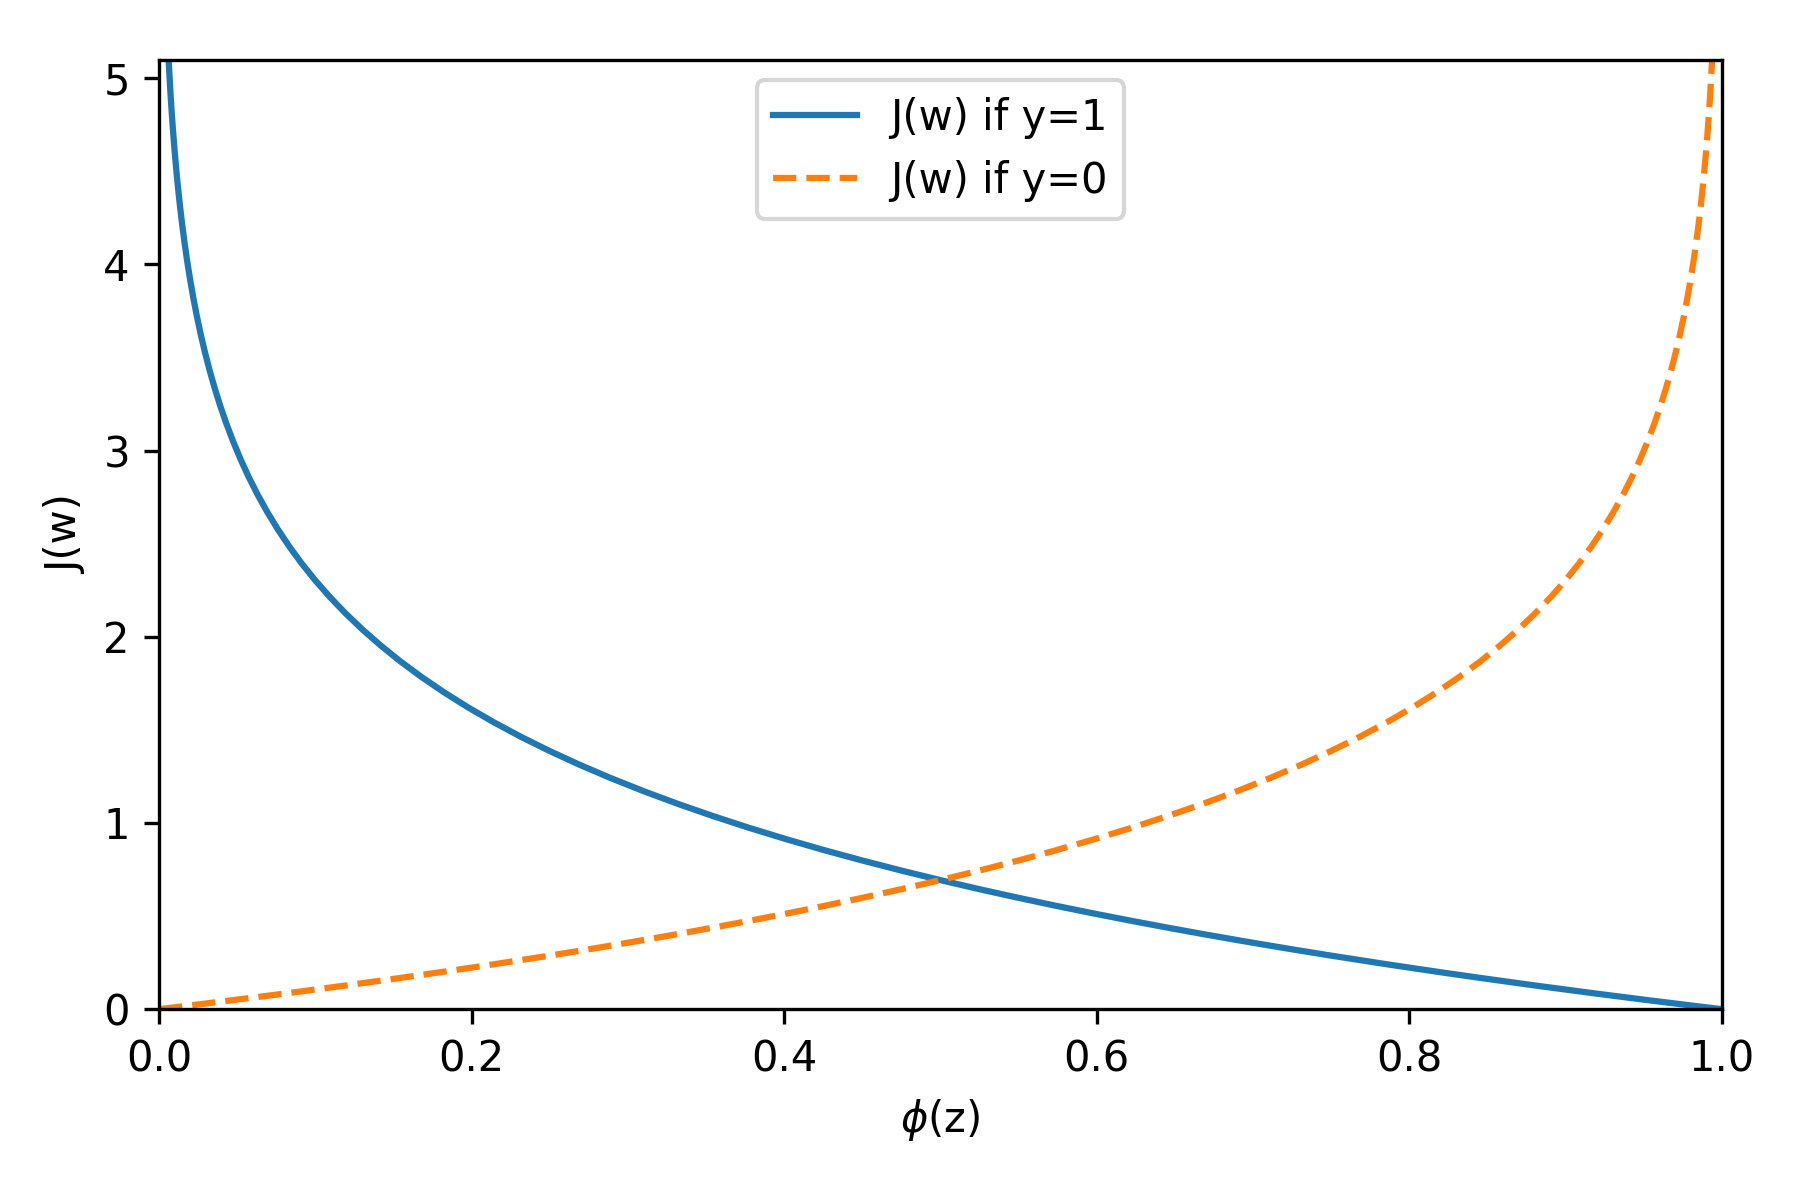
\includegraphics[width=9cm]{images/minimum_log_curve.png}
		\caption{Graphique d'une courbe de régression logistique ajustée aux données $(x_n , y_n)$. \cite[image de]{ml2008python}
		}
		\label{fig:minimum_log_curve}
	\end{figure}
	
	
	
	
	\section{Descente de gradient stochastique}
	Cette section est inspirée des articles écrites par Léon Bottou et al, dans  \cite{bottou2012stochastic} 
	\cite{bottou2010large}
	\cite{framling2004scaled}
	\cite{bottou2018optimization}
	\cite{netrapalli2019stochastic}
	\cite{wijnhoven2010fast}.
	
	\subsection{Descente de gradient (Gradient Descent)}
	
	
	Il a souvent été proposé de minimiser le risque empirique [E] en utilisant la descente de gradient (GD). Chaque itération met à jour les poids w en fonction du gradient de [E] \cite{bottou2012stochastic}.\\
	
	\lipsum[1] \\ 
	
	$$A = \begin{pmatrix}
		x_{11} & x_{12} & x_{13} & \cdots & x_{1n} \\
		x_{21} & x_{22} & x_{23} & \cdots & x_{2n} \\
		\vdots & \vdots & \vdots & \ddots & \vdots \\
		x_{m1} & x_{m2} & x_{m3} & \cdots & x_{mn} 
	\end{pmatrix}$$
	
	
	\lipsum[4]
	\subsubsection{Pourquoi stochastique?}
	Descente de gradient stochastique (SGD) 
	
	L'algorithme de descente de gradient stochastique (SGD) est une simplification drastique. Au lieu de calculer exactement le gradient de E n (f w ), chaque itération estime ce gradient sur la base d'un seul exemple z t pris au hasard \cite{bottou2012stochastic} :
	$$
	{\displaystyle w:=w-\eta \nabla Q(w)=w-{\frac {\eta }{n}}\sum _{i=1}^{n}\nabla Q_{i}(w),}
	$$
	\lipsum[1]	
	\subsection{La convergence de la descente de gradient stochastique}
	\lipsum[1]
	\subsection{Le probleme des minima locaux} \cite[page 291][]{antoine2018apprentissage}????
	
	
	\section{Les optimiseurs SGD}
	\subsection{Perceptron Optimizer}
	
	Le perceptron est un modèle simplifié d'un neurone biologique . Alors que la complexité des modèles de neurones biologiques est souvent nécessaire pour bien comprendre le comportement neuronal, la recherche suggère qu'un modèle linéaire de type perceptron peut produire certains comportements observés dans de vrais neurones.
	
	Un perceptron est une unité de réseau neuronal (un neurone artificiel) qui effectue certains calculs pour détecter des caractéristiques ou une intelligence économique dans les données d'entrée.
	Et aussi en Machine Learnig (apprentissage automatique), le perceptron est un algorithme d'apprentissage supervisé de classificateurs binaires (qui se fait dans la régression logistique). 
	Un classificateur binaire est une fonction qui peut décider si une entrée, représentée par un vecteur de nombres, appartient ou non à une classe spécifique. \cite{freund1999large} Il s'agit d'un type de classificateur linéaire , c'est-à-dire un algorithme de classification qui fait ses prédictions sur la base d'une fonction prédictive linéaire combinant un ensemble de poids avec le vecteur de caractéristiques .
	
	Le premier concept de règle d'apprentissage du perceptron, a été publié par Frank Rosenblatt [??],  basé sur le modèle neuronal MCP(???). 
	
	(F. Rosenblatt, The Perceptron, a Perceiving and Recognizing Automaton. Cornell Aeronautical Laboratory, 1957).
	
	Avec sa règle de perceptron, Rosenblatt a proposé un algorithme qui apprendrait automatiquement les coefficients de poids optimaux qui sont ensuite multipliés par les caractéristiques d'entrée afin de décider si un neurone se déclenche ou non. Dans le cadre de l'apprentissage supervisé et de la classification, un tel algorithme pourrait alors être utilisé pour prédire si un échantillon appartient à une classe ou à l'autre [Python machine learning].
	
	Il est important de noter que la convergence du perceptron n'est garantie que si les deux classes sont linéairement séparables et que le taux d'apprentissage est suffisamment faible. Si les deux classes ne peuvent pas être séparées par une limite de décision linéaire, nous pouvons définir un nombre maximum de passages sur l'ensemble de données d'apprentissage (époques) et/ou un seuil pour le nombre d'erreurs de classification tolérées - le perceptron n'arrêterait jamais de mettre à jour les poids autrement:
	
	\subsection{Neurone linéaire adaptatif (ADALINE)}
	\lipsum[1]
